\section[Lecture4]{\hyperlink{toc}{Lecture 4}}

Thursday, September 18th 2025

\begin{itemize}
    \item For fun Example that depends on cultural assumptions: king comes from family with two kids, what is the probability that the kings sibling is a sister?
    \item $S  = \{ (m,m), (m,f), (f,m), (f,f) \}$
    \item $P(S|K) = \frac{P(SK)}{P(K)} = \frac{\frac{1}{2}}{\frac{3}{4}} = \frac{2}{3}$
\end{itemize}


Distributions of multiple variables
\begin{itemize}
    \item $p(x_1, x_2, \ldots, x_n) $
    \item $S = \mathbb{R}^n$
    \item $\int p(x_1, x_2, \ldots, x_n) \, dx_1 \, dx_2 \, \ldots \, dx_n = 1$
    \item Any $f(\vec{x})$:
    \[ E(f) = \int f(\vec{x}) p(\vec{x}) d \vec{x} \]
    \item $E(x_1) = \int x_1 p(\vec{x}) d \vec{x} = \mu_1$
    \item $E(x_i) = \mu_i$
    \item $V(x_i) \equiv \sigma_i^2 = \int (x_i - \mu_i)^2 p(\vec{x}) d \vec{x}$
    \item Define covariance:
    \[ V_{ij} = E((x_i - \mu_i)(x_j - \mu_j)) \]
    \item $V_{ii} = \sigma_i^2$ variance
    \item $V_{ij} = V_{ji}$ symmetry
    \item $V_{ij} = 0$ independent variables
    \item Looking at expanding the covariance matrix again:
    \begin{align*}
        V_{ij}(\vec{x}) &= E((x_i- \mu_i)(x_j - \mu_j)) \\
        &= E(x_i x_j - \mu_i x_j - \mu_j x_i + \mu_i \mu_j) \\
        &= E(x_i x_j) - \mu_i E(x_j) - \mu_j E(x_i) + \mu_i \mu_j \\
        &= E(x_i x_j) - \mu_i \mu_j - \mu_j \mu_i + \mu_i \mu_j \\
        &= E(x_i x_j) - \mu_i \mu_j
    \end{align*}
    \item So we can saw that $V_{ij} \ge 0$
    \item $V_{ij}$ can't be -ve, 0, or +ve
    \item We define the correlation coefficient:

    \[ \rho(x_i, x_j) = \rho_{ij} = \frac{V_{ij}}{\sqrt{V_{ii}} \sqrt{V_{jj}}} = \frac{V_{ij}}{\sigma_i \sigma_j} \]

    \item We find the $-1 \le \rho_{ij} \le 1$
    \item Independent variables
    \item Random variables $x_i, \dots, x_n$ are independent if: joint pdf factorizes.
    \item $p(x_1, \ldots, x_n) = p_1(x_1) p_2(x_2) \ldots p_n(x_n)$
    \item Independent variables are uncorrelated:
    \begin{align*}
        E(x_i x_j) &= \int x_i x_j p(\vec{x}) d \vec{x} \\
        &= \int x_i x_j p_1(x_1) \ldots p_n(x_n) dx_1 \ldots dx_n \\
        &= \int x_i p_i(x_i) dx_i \int x_j p_j(x_j) dx_j \int p_2(x_2) dx_2 \ldots \int p_n(x_n) dx_n = \mu_i \mu_j
    \end{align*}

    \[ V_{ij} = E(x_i x_j) - \mu_i \mu_j\]
    In case of independent variables:

    \[ V_{ij} = \mu_i \mu_j - \mu_i \mu_j = 0 \]

    \item Independent variables are uncorrelated but uncorrelated variables are not necessarily independent.
    \item 100 \% correlation: 
    \item $ x = \text{Uniform} [-1, 1]$, plot distribution from $-1$ to $1$.
    \item $y=x$:
    \item $V_{ij} = E(xy)-E(x)E(y)= E(x^2) = \int_{-1}^{1} x^2 \frac{1}{2} dx = \frac{1}{3} \neq 0$
    \item $y=|x|$:
    \item $E(xy) = \int_{-1}^{0} x(-x) p(x) d(x)   + \int_0^{1}  x x p(x)dx$
    \item $ E(xy) = \int_0^{1} x^2 \frac{1}{2} dx - \int_{-1}^{0} x^2 \frac{1}{2} dx = \frac{1}{6} - \frac{1}{6} = 0$

    \item Marginal distributions:
    
    \item Joint pdf, $p(x_1, x_2, \ldots, x_n)$
    \item The marginal prob density functions 
    \[ f_1(x_1) = \int p(x_1, x_2, \ldots, x_n) dx_2 dx_3\ldots dx_n \]

    \item If variables are independent:
    
    \begin{align*}
        f_1(x_1) &= \int p(x_1, x_2, \ldots, x_n) dx_2 \ldots dx_n \\
        &= p_1(x_1) \int p_2(x_2) dx_2 \int p_3(x_3) dx_3 \ldots \int p_n(x_n) dx_n \\
        &= p_1(x_1) \cdot 1 \cdot 1 \cdot \ldots \cdot 1 = p_1(x_1)
    \end{align*}

    \item Something we need to know, because we do it all the time! :
    \begin{itemize}
        \item Change of variables of P
        \item Calculate new $V_{ij}$ under new variables
    \end{itemize}

    \item Let x be a random variable with pdf $f(x)$
    \item Let $y$ be some function
    \item 1st: y is 1-to-1 with f    
    
    \begin{figure}[h]
        \centering
        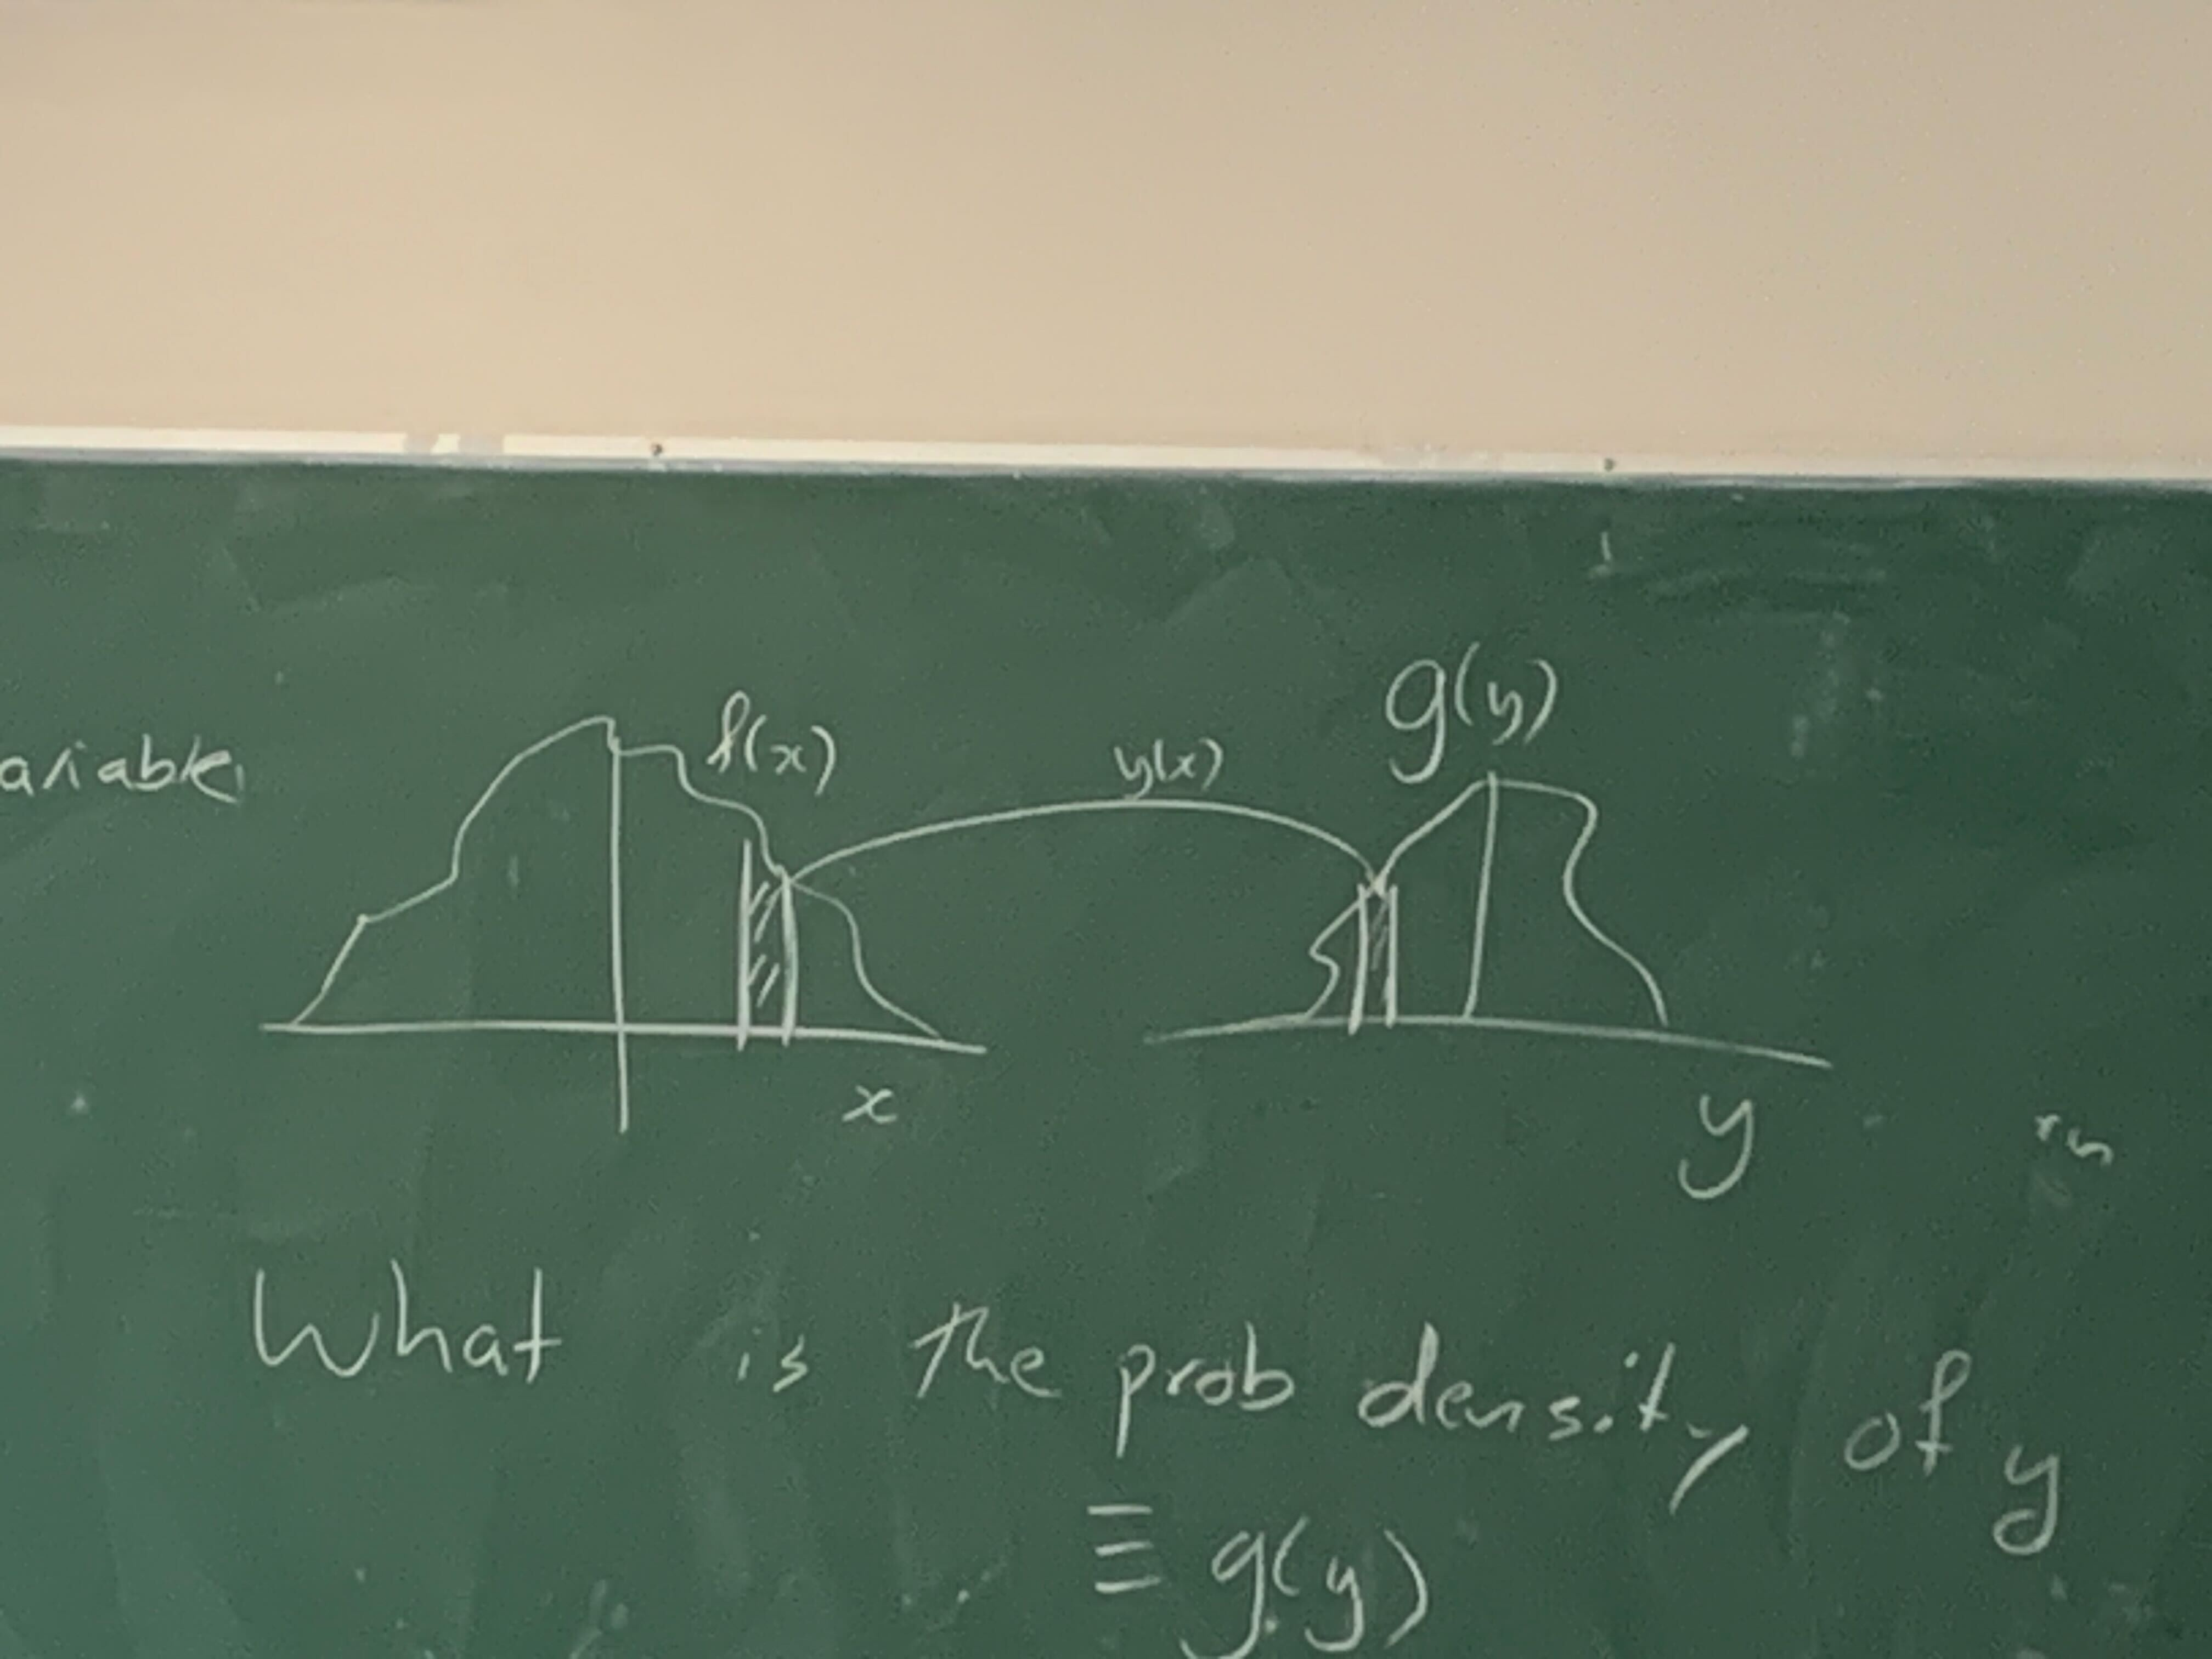
\includegraphics[width=0.4\textwidth]{Images/lec4-fig1.jpg}
        \caption{1-to-1 function}
        \label{fig:fig1}
    \end{figure}
    \item What is the prob density of y ... $\equiv g(y)$ ?
    
    \item Conservation of probability:
    \item $f(x) dx = g(y) dy$
    \item $g(y) = f(x) \left| \frac{dx}{dy} \right|$
    \[ \boxed{ f(x) \left| \frac{dx}{dy} \right| = g(y) } \]

    \item If y not 1-to-1:
    \item Sum over at 1 segments that map to same y.
    \item Example $f(x)$ = uniform on $[0,1] = 1$
    \item Let $y(x) = \frac{-1}{\lambda} \ln(x)$
    \item $\frac{dy}{dx} = \frac{-1}{\lambda x}$
    \item $\frac{dx}{dy} = -\lambda x$ 
    \item $-\lambda x = \ln{x}$
    \item $e^{-\lambda y} = x$
    \item $\lambda > 0 \Rightarrow \frac{dx}{dy} = - \lambda x = -\lambda e^{-\lambda y} $
    \item $ g(y) = f(x) \left| \frac{dx}{dy} \right| = 1 \cdot \lambda e^{-\lambda y} = \lambda e^{-\lambda y}$
    \item If have a variables $\{x_i\}$ and transform to n $\{y_i\}$
    \item Region $\mathbb{R}$ in x-space maps to region $\mathbb{R'}$ in y-space.
    \[ \int_{\mathbb{R}} f(\vec{x}) d\vec{x} = \int_{\mathbb{R'}} f(\vec{x}(\vec{y}))(\vec{y}) \left|\pdv{\vec{x}}{\vec{y}} \right| d\vec{y} \]
    \[ g(\vec{y}) = f(\vec{x}(\vec{y})) \left| J \right| \]
    \item Where $\left|\pdv{\vec{x}}{\vec{y}} \right|$ is the Jacobian determinant of the transformation.
    \item Jacobian matrix J:
    \[ J = \begin{bmatrix}
        \pdv{x_1}{y_1} & \pdv{x_1}{y_2} & \ldots & \pdv{x_1}{y_n} \\
        \pdv{x_2}{y_1} & \pdv{x_2}{y_2} & \ldots & \pdv{x_2}{y_n} \\
        \vdots & \vdots & \ddots & \vdots \\
        \pdv{x_n}{y_1} & \pdv{x_n}{y_2} & \ldots & \pdv{x_n}{y_n}
    \end{bmatrix} \]
    \item Change to polar:
    \item $x = r \cos{\theta}$
    \item $y = r \sin{\theta}$
    \item $P'(r, \theta) = ? = p(x,y) \left| \pdv{(x,y)}{(r,\theta)} \right|$
    
    \item $ \pdv{x}{r} = \cos{\theta}$
    \item $ \pdv{y}{r} = \sin{\theta}$
    \item $ \pdv{x}{\theta} = -r \sin{\theta}$
    \item $ \pdv{y}{\theta} = r \cos{\theta}$
    
    \item $J = \begin{bmatrix}
        \cos{\theta} & -r \sin{\theta} \\
        \sin{\theta} & r \cos{\theta}
    \end{bmatrix}$

    \item $ J = r \cos^2{\theta} + r \sin^2{\theta} = r$
    \item $p'(r, \theta) = \frac{r}{\pi} dr d\theta$

\end{itemize}
